\subsection{Magnification-Arbitrary Network (MetaSR \cite{MetaSR})}
The limitation of SR task using fixed integer scales are:
\begin{itemize}
    \item real application may be necessary upsampling on continues scales (such as in medical imaging, satellite imaging, \dots ).
    \item if the network is trained on a specific scale and is not capable to output intermediate scales (such as \cite{LapSRN}) then there are also training cost and memory cost.
\end{itemize}

In order to overcame fixed integer problems \cite{MetaSR} exploit \textbf{meta-learning} in order to be able to use decimal scales.

\subsubsection{Background}

The idea is used in \cite{ParametrizedImageOperator} where research trained different parametrized operator ( a generic function that transforms an image based on parameters ) using a neural network exploiting meta-learning.

There are two networks \Cref{PIO:model}:
\begin{itemize}
    \item $N_{base}$ which applies the mapping
    \item $N_{weights}$ which learns the weights to use inside convolutions in $N_{base}$ based on the parameters 8$\vec{\gamma}$) given to the function. 
\end{itemize}
that are learned together end-to-end: 
$$
L = \Vert N_{base}(N_{weight}(\vec{\gamma},I,E)) - f(I,\vec{\gamma}) \Vert_2^2
$$
\begin{figure}
    \centering
    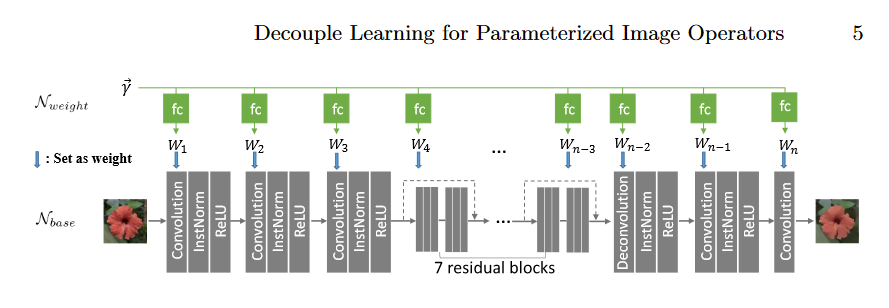
\includegraphics[width=0.8\textwidth, keepaspectratio]{paramsimageoperatormodel.png}
    \caption{Parametrized Image Operator network.}\label{PIO:model}
\end{figure}

\subsubsection{Architecture}
\begin{figure}
    \centering
    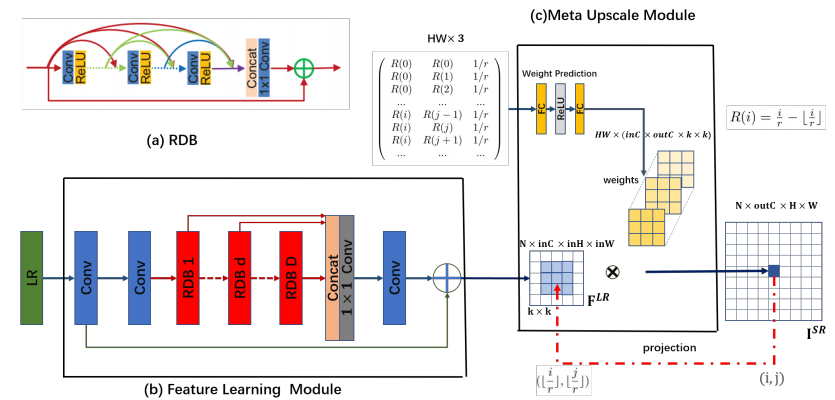
\includegraphics[width=\textwidth, keepaspectratio]{metasr-model.png}
    \caption{Meta-SR architecture.}\label{metasr:model}
\end{figure}

The \textbf{Feature Learning Module} extracts features at low resolution which are used by the \textbf{Meta Upscale Module} for generating the SR image.

The \textit{Feature Learning Module} can be any state-of-the-art network while \textit{Meta Upscale Module} replace the upsampling layer in the selected network.

\paragraph{Meta Upscale Module}

The \textbf{Meta Upscale Module} contains three different modules:
\begin{itemize}
    \item \textbf{location projector} which project pixels from HR images to LR images: $(i',j') = T(i,j) = (\lfloor\frac{i}{r}\rfloor,\lfloor\frac{j}{r}\rfloor)$ where $(i,j)$ are pixels in the HR image and $(i',j')$ are pixels in the LR image.
    \begin{figure}[h]
        \centering
        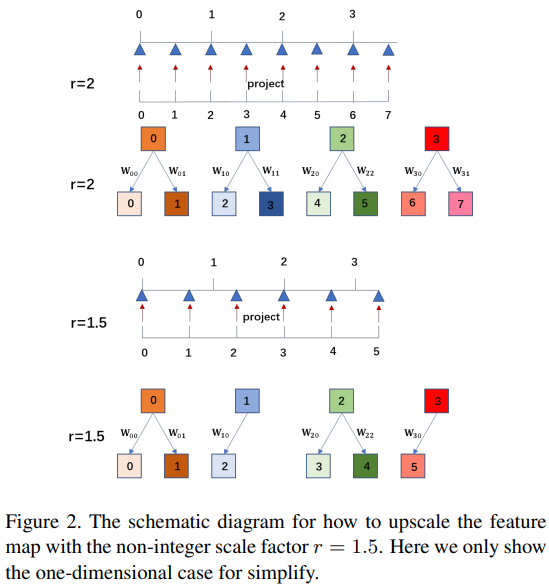
\includegraphics[scale=0.5]{metasr-location-projector.png}
        \caption{Location projector: each pixel in the SR image (bottom row) has an unique pixel in the LR image (top row).}
    \end{figure}

    \item \textbf{weight prediction} which predicts the weights of the kernel for each pixel $W(i,j)=\phi(v_{ij},\theta)$ where $\phi$ is a network with fully connected layers (2 with 256 hidden units ad ReLu as activation).
    
    $v_{ij}$ is a vector of pixel offset locations:
    
    $v_{ij} = (\frac{i}{r}-\lfloor\frac{i}{r}\rfloor, \frac{j}{r}-\lfloor\frac{j}{r}\rfloor, \frac{1}{r})$

    (in order to allow the network to distinguish between different scales $\frac{1}{r}$ is inserted in the vector because for example the pixel (i,j) in a 2x image has the same projection and the same weights of the pixels (2i,2j) in a 4x image)
    
    \item \textbf{feature mapping} which use the features extracted by the \textit{Feature Module} and the weights predicted by the \textit{Weight Prediction} module for reconstructing the HR image:
    
    $\Phi(F^{LR}(i',j'), W(i,j)) = F^{LR}(i',j') \ast W(i,j)$ (in practice it does the convolution of the features map with the kernel for getting an intensity or rgb values)
\end{itemize}



\subsubsection{Results}

\begin{figure}
    \centering
    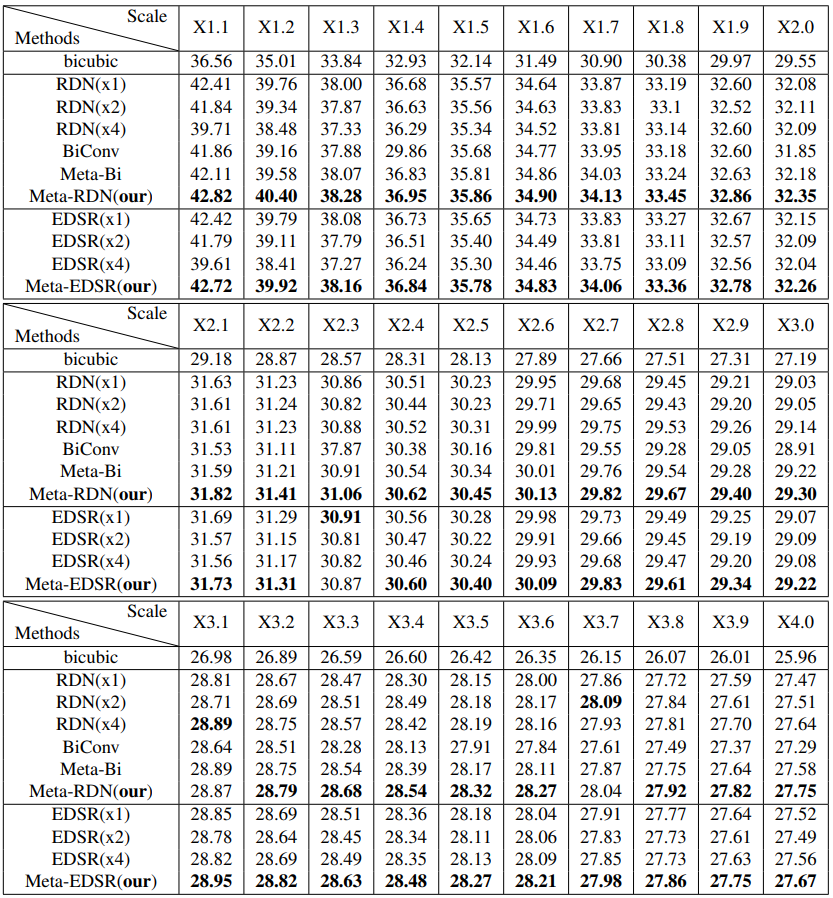
\includegraphics[width=\textwidth, keepaspectratio]{metasr-results1.png}
    \caption{Results on Meta-SR}\label{metasr:results}
\end{figure}

\paragraph{Results with decimal scales}
From the results [\Cref{metasr:results}] Meta-SR, and in particular the \textbf{Meta upscaling module}, performs better since Meta-RDN performs better than Meta-Bi (both are learning the weights for upscaling) which perform better than BiConv (where weights are the same for each scale).

The baseline are:
\begin{itemize}
    \item bicubic
    \item RDN(x1) and EDSR(x1): LR image is upscaled by $r$ and processed by the network
    \item RDN(x$k$) and EDSR(x$k$): LR image is processed by the network which apply a upscaling by $k$ then the HR image is downscaled by $\frac{r}{k}$
    \item BiConv: interpolation of the final feature maps and same convolution for all scales.
    \item Meta-Bi: interpolation of the final feature maps but use different weights for each scale using the Weight Prediction Network. 
\end{itemize}

\paragraph{Comparison between RDN and Meta-RDN}
\begin{figure}
    \centering
    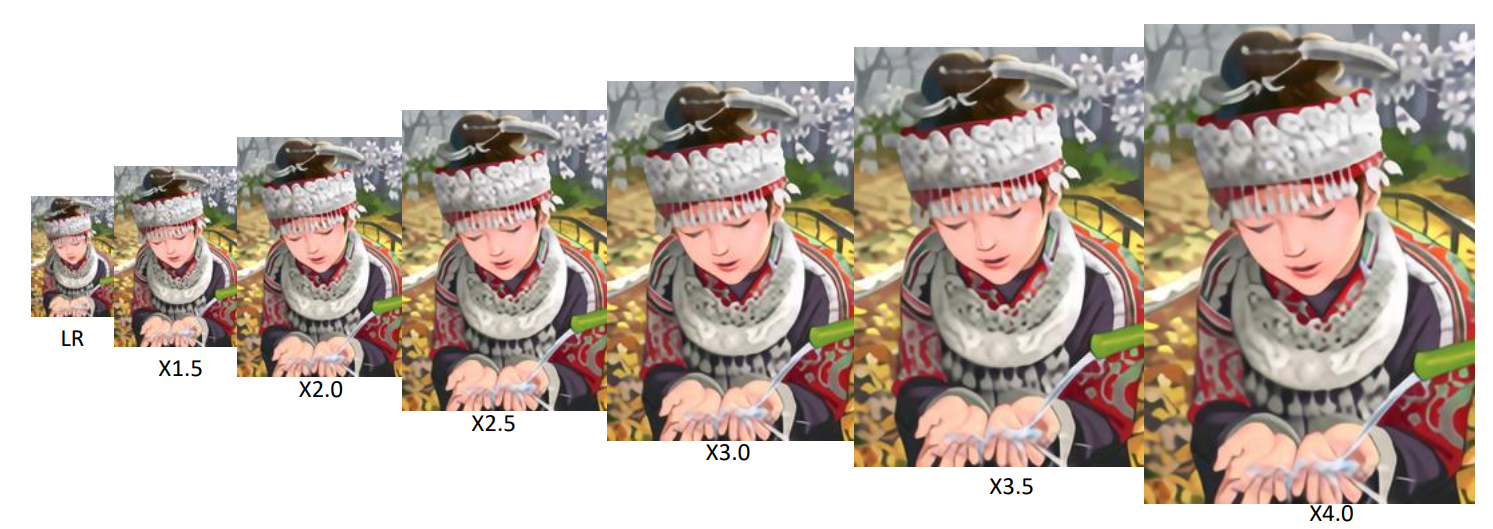
\includegraphics[width=\textwidth, keepaspectratio]{metasr-qualitative.png}
    \caption{Meta-SR applied for different scales to a single image.}
\end{figure}

\begin{figure}
    \centering
    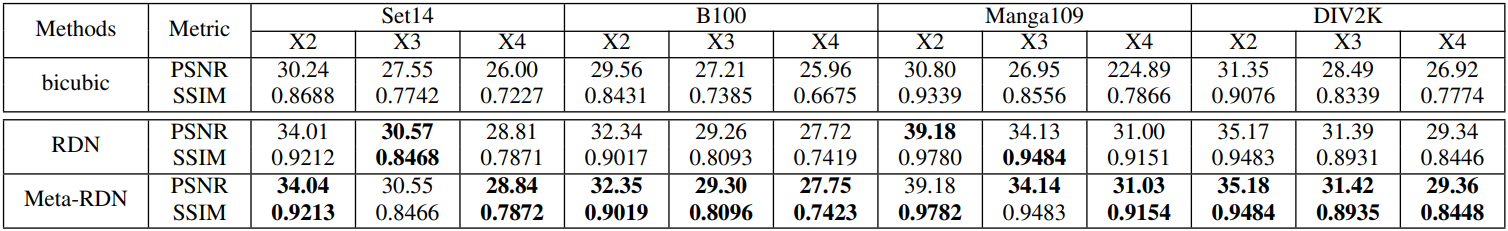
\includegraphics[width=\textwidth, keepaspectratio]{metasr-results-comparison.png}
    \caption{Meta-SR versus RDN.}
\end{figure}

\begin{figure}
    \centering
    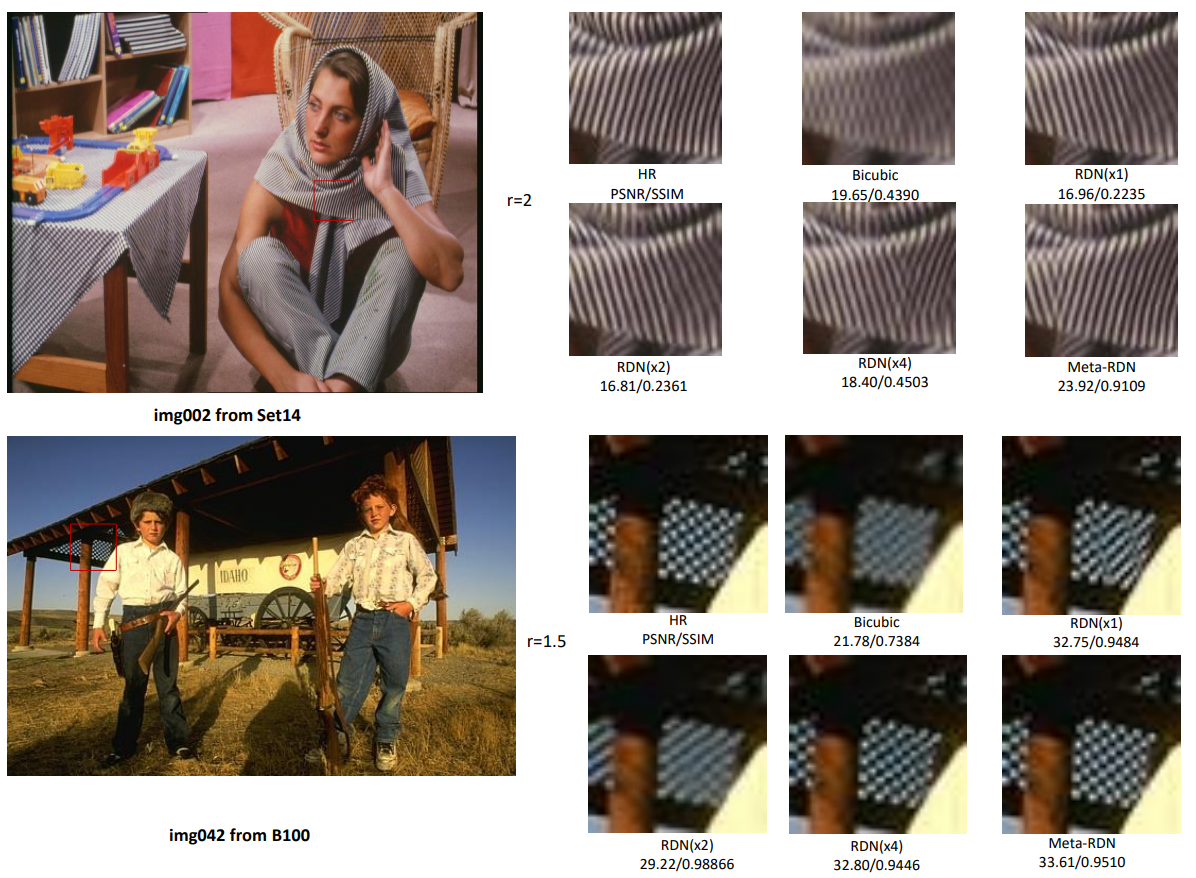
\includegraphics[width=\textwidth, keepaspectratio]{metasr-qualitative-comparison.png}
    \caption{The visual comparison with four baselines. Our MetaRDN has better performance.}
\end{figure}

Overall Meta-SR performs better than RDN on decimal scales.